\documentclass[review]{elsarticle}

% =============================================================================
% Packages
% =============================================================================
\usepackage[utf8]{inputenc}
\usepackage[T1]{fontenc}
\usepackage{amsmath,amssymb}
\usepackage{siunitx}
\usepackage{graphicx}
\usepackage{subcaption}
\usepackage{booktabs}
\usepackage[pdfencoding=auto,psdextra]{hyperref}
\usepackage{lineno}

% Fix duplicate page destination warning with elsarticle review mode
\hypersetup{pageanchor=false}
\AtBeginDocument{\hypersetup{pageanchor=true}}

% SI units configuration
\sisetup{
  per-mode=symbol,
  group-separator={,},
}

% Line numbering (required for JSV review submission)
\linenumbers

% =============================================================================
% Metadata
% =============================================================================
\journal{Journal of Sound and Vibration}

\begin{document}

\begin{frontmatter}

\title{Modal Analysis of a Fluid-Filled Viscoelastic Oblate Spheroidal Shell:
Implications for the Existence of the ``Brown Note''}

\author[msr]{Jonathan Mace\corref{cor1}}
\cortext[cor1]{Corresponding author}
\ead{jonathanmace@microsoft.com}

\author[auckland]{Brian R.\ Mace}
\ead{br.mace@auckland.ac.nz}

\author[springbank]{Springbank 10 Year Old\fnref{fn1}}
\fntext[fn1]{Non-sentient author. Contribution limited to inspiration, courage,
  and a pleasantly peaty finish. The distillery neither endorses nor is aware of
  this work.}

\author[github]{GitHub Copilot CLI\fnref{fn2}}
\fntext[fn2]{Large language model. Performed literature review, analytical
  computation, code development, figure generation, and manuscript drafting
  under human supervision.}

\affiliation[msr]{
  organization={Microsoft Research},
  city={Redmond, WA},
  country={United States}
}

\affiliation[auckland]{
  organization={Acoustics Research Centre, Department of Mechanical and
    Mechatronics Engineering, University of Auckland},
  city={Auckland},
  country={New Zealand}
}

\affiliation[springbank]{
  organization={Springbank Distillery},
  city={Campbeltown, Argyll},
  country={Scotland}
}

\affiliation[github]{
  organization={GitHub, Inc.},
  city={San Francisco, CA},
  country={United States}
}

\begin{highlights}
\item Mechanical--airborne coupling disparity of $\sim$$10^4$ explains gastrointestinal vibration asymmetry
\item Fluid-filled viscoelastic shell model predicts abdominal resonance at 4--10 Hz (matches ISO~2631)
\item Breathing mode at $\sim$2500 Hz; flexural modes at infrasonic frequencies
\item Airborne coupling penalised by $(ka)^n$; negligible at 120 dB SPL ($\xi = \SI{0.014}{\micro\metre}$)
\item Monte Carlo UQ confirms robustness; Sobol $S_T = 0.86$ for elastic modulus
\end{highlights}

\begin{abstract}
Whole-body vibration at \SIrange{4}{8}{\hertz} causes well-documented
gastrointestinal disturbances, yet airborne sound at the same frequencies does
not---even at extreme intensities.  We resolve this long-standing asymmetry
by modelling the human abdomen as a fluid-filled viscoelastic oblate
spheroidal shell and quantifying the coupling efficiency of both excitation
pathways within a common energy-budget framework.

The model reveals two distinct mode families.  The breathing mode ($n=0$),
dominated by the fluid bulk modulus, sits near \SI{2500}{\hertz} and is
irrelevant at infrasonic frequencies.  Flexural modes ($n \geq 2$), in which
the shell deforms without compressing the enclosed fluid, fall in the
\SIrange{4}{10}{\hertz} range for relaxed musculature---consistent with
abdominal resonance data from ISO~2631.  At these frequencies, however, the
acoustic wavelength exceeds \SI{49}{\metre}, placing the abdomen deep in the
Rayleigh regime ($ka \approx 0.01$).  The resulting $(ka)^n$ geometric
penalty, compounded by the air--tissue impedance mismatch, reduces airborne
coupling by approximately four orders of magnitude.  Energy-consistent
analysis yields wall displacements of \SI{0.014}{\micro\metre} at
\SI{120}{\decibel} SPL---far below known mechanotransduction thresholds.
Mechanical vibration, transmitted through the skeleton, suffers neither penalty
and produces displacements roughly $4.6 \times 10^4$ times larger at
occupational exposure levels.  Monte Carlo uncertainty quantification confirms
this coupling disparity across physiologically realistic parameter ranges
(Sobol $S_T = 0.86$ for elastic modulus).

The result explains the empirical record quantitatively and, incidentally,
settles the ``brown note'' question: the abdominal resonance invoked by the
myth is genuine, but airborne sound is the wrong mechanism by four orders of
magnitude.
\end{abstract}

\begin{keyword}
fluid-filled shell vibration \sep viscoelastic oblate spheroid \sep
infrasound \sep whole-body vibration \sep acoustic--structural coupling \sep
ISO~2631
\end{keyword}

\end{frontmatter}

% =============================================================================
% Section 1: Introduction
% =============================================================================
\section{Introduction}
\label{sec:introduction}

Low-frequency acoustic and vibrational exposures are ubiquitous in
occupational and environmental settings---from wind turbines and heavy
machinery to transport vehicles and industrial plant.  The human body is known
to exhibit resonance phenomena in the \SIrange{4}{8}{\hertz} range under
whole-body vibration, with the abdominal viscera identified as the primary
resonant subsystem \cite{iso2631,griffin1990handbook}.

A persistent claim in popular culture holds that a specific infrasonic
frequency in the \SIrange{5}{9}{\hertz} range---the so-called ``brown
note''---can cause involuntary loss of bowel control through resonance of the
abdominal cavity.  Despite widespread repetition, no rigorous scientific study
has confirmed this claim, and it has been explicitly debunked in controlled
experiments \cite{Leventhall2007}.

However, the complete absence of a \emph{quantitative mechanistic analysis}
leaves the question incompletely resolved.  No study has:
\begin{enumerate}
  \item derived abdominal cavity eigenfrequencies from first-principles
    shell theory with proper fluid--structure coupling;
  \item quantified the airborne acoustic coupling coefficient for flexural
    modes in the long-wavelength limit; or
  \item compared airborne and mechanical excitation pathways using a common
    modal framework.
\end{enumerate}

The present work addresses all three gaps. We model the abdomen as a
fluid-filled viscoelastic oblate spheroidal shell and derive natural
frequencies for both breathing ($n=0$) and flexural ($n \geq 2$) mode
families.  We then compare the efficiency of airborne acoustic coupling
(subject to a $(ka)^n$ penalty) against mechanical whole-body vibration
coupling (which bypasses this penalty entirely).

The central finding is that the coupling disparity between these two
pathways---a factor of $10^3$--$10^4$---quantitatively explains why
whole-body vibration at \SIrange{4}{8}{\hertz} produces gastrointestinal
effects while airborne infrasound at comparable frequencies does not.

The remainder of this paper is organised as follows. Section~\ref{sec:formulation}
develops the mathematical formulation for the fluid-filled viscoelastic shell,
including both breathing and flexural mode families and the two coupling
pathways. Section~\ref{sec:results} presents a comprehensive parametric study
and validates the model against ISO~2631 data. Section~\ref{sec:coupling}
quantifies the airborne--mechanical coupling disparity.
Section~\ref{sec:discussion} interprets the results and discusses limitations,
and Section~\ref{sec:conclusion} summarises the conclusions.


% =============================================================================
% Section 2: Mathematical Formulation (the core contribution)
% =============================================================================
\section{Mathematical Formulation}\label{sec:formulation}

\subsection{Model Geometry and Assumptions}\label{sec:geometry}

The human abdominal cavity is idealised as an oblate spheroidal shell of
semi-major axes $a$ (equatorial, in the lateral and cranio-caudal directions)
and semi-minor axis $c$ (antero-posterior), with $c < a$.  The shell has uniform
wall thickness $h$ and is completely filled with an inviscid, irrotational
fluid of density $\rho_f$ and bulk modulus $K_f$.  Following standard practice
in fluid-filled shell analysis \cite{Junger1986,lamb1882} and recent
experimental and analytical studies of pressurised elastic shells
\cite{Kuo2015,Ghaheri2022}, an
equivalent-sphere radius is defined via
\begin{equation}\label{eq:Req}
  R_\mathrm{eq} = (a^2 c)^{1/3},
\end{equation}
which preserves the cavity volume, $V = \tfrac{4}{3}\pi a^2 c$.  This
approximation is exact for a sphere ($c = a$) and introduces errors of order
$(1 - c/a)^2$ for the eigenfrequencies at moderate aspect ratios ($c/a \gtrsim
0.5$).  Table~\ref{tab:params} lists the baseline geometric and material
parameters with physiological justification.

The thin-shell assumption ($h/R_\mathrm{eq} \ll 1$) is satisfied: for
$h = 10$\,mm and $R_\mathrm{eq} \approx 157$\,mm, $h/R \approx 0.06$.  The
Love--Kirchhoff hypothesis (normals remain straight and normal to the
deformed mid-surface) is therefore applicable.  This linear framework remains
the standard starting point even in modern reviews of nonlinear shell
vibration, which treat geometric nonlinearities as amplitude corrections to
the same modal backbone \cite{Alijani2014}.

\begin{table}[htbp]
  \centering
  \caption{Baseline model parameters with physiological justification.}
  \label{tab:params}
  \begin{tabular}{lcccl}
    \hline
    Parameter & Symbol & Value & Unit & Source \\
    \hline
    Semi-major axis & $a$ & 0.18 & m & Anthropometric mean \\
    Semi-minor axis & $c$ & 0.12 & m & $c/a \approx 0.67$ \\
    Wall thickness & $h$ & 0.010 & m & Composite wall \\
    Elastic modulus & $E$ & 0.1 & MPa & Representative of reported measurements \cite{Deeken2017} \\
    Poisson's ratio & $\nu$ & 0.45 & --- & Near-incompressible modelling convention \cite{Spadoni2024} \\
    Wall density & $\rho_w$ & 1100 & kg/m$^3$ & Soft tissue \\
    Fluid density & $\rho_f$ & 1020 & kg/m$^3$ & Abdominal fluid \\
    Fluid bulk modulus & $K_f$ & 2.2 & GPa & Water at 37$^\circ$C \\
    Intra-abdominal pressure & $P_\mathrm{iap}$ & 1000 & Pa & Representative resting clinical measurement \cite{Novak2021} \\
    Loss tangent & $\eta$ & 0.25 & --- & Representative review value \cite{Sack2023} \\
    \hline
  \end{tabular}
\end{table}

\begin{figure}[htbp]
  \centering
  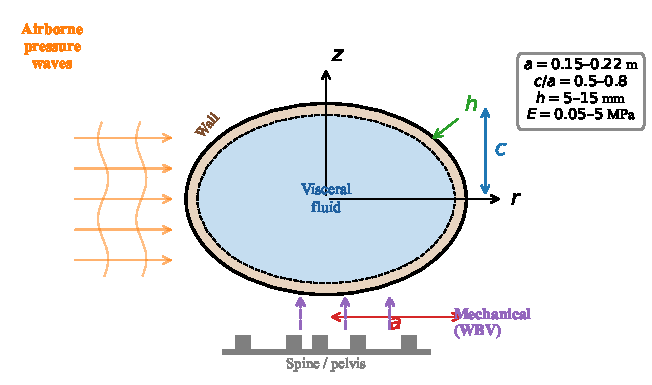
\includegraphics[width=\textwidth]{../data/figures/fig_geometry_schematic.pdf}
  \caption{Oblate spheroidal shell model of the human abdominal cavity,
  showing the two excitation pathways: airborne acoustic pressure (left)
  and mechanical whole-body vibration transmitted through the skeleton (right).
  Dimensions correspond to the baseline parameters in Table~\ref{tab:params}.}
  \label{fig:geometry}
\end{figure}

Figure~\ref{fig:geometry} illustrates the model geometry and the two excitation
pathways.  The abdominal wall is modelled as a Kelvin--Voigt viscoelastic material with
complex modulus
\begin{equation}\label{eq:Estar}
  E^* = E(1 + i\eta),
\end{equation}
where $\eta$ is the loss tangent.  For small damping, the quality factor is
$Q = 1/\eta$ and the viscous damping ratio is $\zeta = \eta/2 = 1/(2Q)$.  The
flexural rigidity of the shell is
\begin{equation}\label{eq:D}
  D = \frac{Eh^3}{12(1 - \nu^2)}.
\end{equation}
These baseline values are not arbitrary.  The canonical modulus
$E = \SI{0.1}{\mega\pascal}$ is representative of direct abdominal-wall
measurements compiled by Deeken and Lake \cite{Deeken2017};
$\nu = 0.45$ follows the nearly incompressible modelling convention adopted in
recent abdominal-wall finite-element studies \cite{Spadoni2024}; resting
intra-abdominal pressures of 5--12\,mmHg correspond to approximately
\SIrange{0.67}{1.60}{\kilo\pascal}, so
$P_\mathrm{iap} = \SI{1.0}{\kilo\pascal}$ is representative of direct clinical
measurements \cite{Novak2021}; and modern elastography reviews place the
soft-tissue loss tangent broadly in the 0.1--0.4 range, making
$\eta = 0.25$ consistent with the range reported for soft tissue
\cite{Sack2023}.  Published values of $\eta$ for abdominal
soft tissue range from 0.15 to 0.40 at low frequencies
\cite{parker2011imaging}, corresponding to $Q = 2.5$--$6.7$.  The baseline
value $\eta = 0.25$ ($Q = 4.0$, $\zeta = 0.125$) represents a central estimate.


\subsection{Breathing Mode (\texorpdfstring{$n = 0$}{n = 0})}\label{sec:breathing}

The breathing mode is a spatially uniform radial oscillation in which the shell
displaces by $\xi$ at every point.  The associated volumetric strain is
$\Delta V/V = 3\xi/R$, which compresses the contained fluid.  Two restoring
forces act on the shell:

\paragraph{Membrane stiffness.}
For the uniform expansion of a thin spherical shell,
\begin{equation}\label{eq:kshell}
  k_\mathrm{shell} = \frac{2Eh}{R^2(1 - \nu)}.
\end{equation}

\paragraph{Fluid volumetric stiffness.}
The pressure increment due to fluid compression is $\Delta p = K_f \Delta V /
V = 3K_f \xi / R$.  The restoring force per unit displacement per unit area is
\begin{equation}\label{eq:kfluid}
  k_\mathrm{fluid} = \frac{3K_f}{R}.
\end{equation}
With $K_f = 2.2$\,GPa and $R = 0.157$\,m, $k_\mathrm{fluid} = 4.2 \times
10^{10}$\,Pa/m, which exceeds the membrane stiffness ($k_\mathrm{shell}
\approx 1.5 \times 10^5$\,Pa/m) by five orders of magnitude.  \emph{The
breathing mode is entirely dominated by the fluid bulk modulus.}

The effective mass per unit area includes the shell wall and the fluid added
mass for the $n = 0$ mode:
\begin{equation}\label{eq:m0}
  m_\mathrm{eff}^{(0)} = \rho_w h + \rho_f R.
\end{equation}

The breathing mode frequency is therefore
\begin{equation}\label{eq:f0}
  f_0 = \frac{1}{2\pi}\sqrt{\frac{k_\mathrm{shell} + k_\mathrm{fluid}}
  {\rho_w h + \rho_f R}} \approx 2500\;\text{Hz},
\end{equation}
which lies in the kilohertz range and is irrelevant to infrasonic exposure.
This result is robust to material property variations because $k_\mathrm{fluid}
\gg k_\mathrm{shell}$ for any realistic shell stiffness.


\subsection{Flexural Modes (\texorpdfstring{$n \geq 2$}{n >= 2})}\label{sec:flexural}

Flexural modes involve shape changes (oblate--prolate oscillation for $n = 2$,
trilobed for $n = 3$, etc.)\ that preserve the enclosed volume to leading
order.  The fluid therefore does \emph{not} act as a volumetric spring; it
contributes only added mass.

Following Lamb \cite{lamb1882} and Junger \& Feit
\cite{Junger1986}, with subsequent validation in modern pressurised-shell
studies \cite{Kuo2015,Ghaheri2022}, the flexural mode of order $n$ has three contributions
to the restoring force per unit area.  (An analogous modal decomposition
for fluid-filled elastic tubes in biological contexts was developed by
Heil~\cite{Heil1996}.)

\paragraph{Bending stiffness.}
\begin{equation}\label{eq:Kbend}
  K_\mathrm{bend} = \frac{n(n-1)(n+2)^2 D}{R^4}.
\end{equation}

\paragraph{Membrane stiffness.}
\begin{equation}\label{eq:Kmemb}
  K_\mathrm{memb} = \frac{Eh}{R^2}\,\lambda_n,
  \qquad \lambda_n = \frac{n^2 + n - 2 + 2\nu}{n^2 + n + 1 - \nu}.
\end{equation}

\paragraph{Pre-stress stiffness.}
The static intra-abdominal pressure $P$ produces a pre-stress in the
shell membrane that stiffens flexural modes:
\begin{equation}\label{eq:Kpre}
  K_P = \frac{P}{R}(n-1)(n+2).
\end{equation}

The fluid added mass per unit area for mode $n$ is
\begin{equation}\label{eq:madd}
  m_\mathrm{add}^{(n)} = \frac{\rho_f R}{n},
\end{equation}
giving a total effective mass of
\begin{equation}\label{eq:meff}
  m_\mathrm{eff}^{(n)} = \rho_w h + \frac{\rho_f R}{n}.
\end{equation}

The natural frequency of flexural mode $n$ is
\begin{equation}\label{eq:fn}
  \omega_n^2 = \frac{K_\mathrm{bend} + K_\mathrm{memb} + K_P}
                    {m_\mathrm{eff}^{(n)}},
  \qquad f_n = \frac{\omega_n}{2\pi}.
\end{equation}

For the baseline parameters (Table~\ref{tab:params}), $f_2 = 4.0$\,Hz,
$f_3 = 6.3$\,Hz, and $f_4 = 8.9$\,Hz (Figure~\ref{fig:modes}).  (The $n = 1$
mode corresponds to rigid-body translation and has zero natural frequency for
a free shell; it is therefore excluded.)  These lie squarely in the 4--10\,Hz
range reported for abdominal resonance in ISO~2631 \cite{iso2631} and in the
experimental studies of Kitazaki \& Griffin \cite{kitazaki1998resonance} and
Mansfield \cite{mansfield2005human}.

\begin{figure}[htbp]
  \centering
  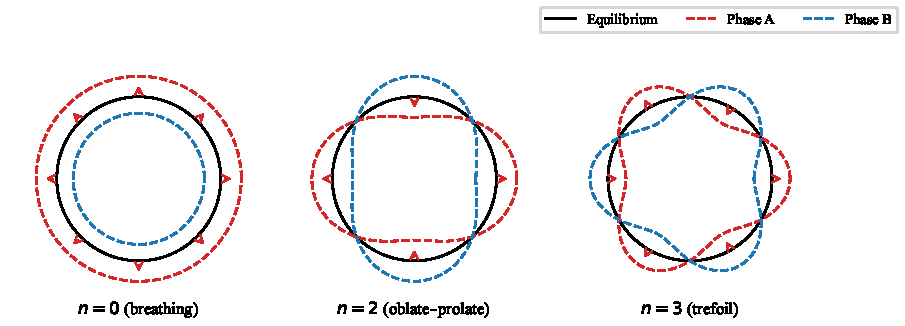
\includegraphics[width=\textwidth]{../data/figures/fig_mode_shapes.pdf}
  \caption{Schematic cross-sections of the first three mode families.
  The breathing mode ($n=0$) involves uniform radial expansion against
  the fluid bulk modulus.  Flexural modes ($n=2, 3$) deform the shell
  shape without significant volume change; the enclosed fluid acts as
  added mass only.}
  \label{fig:modes}
\end{figure}


\subsection{Airborne Acoustic Coupling}\label{sec:airborne}

We now quantify the excitation of flexural modes by an incident airborne
acoustic field.  At $f_2 \approx 4$\,Hz, the acoustic wavelength in air is
$\lambda \approx 87$\,m, so the dimensionless wavenumber is
\begin{equation}\label{eq:ka}
  ka = \frac{2\pi f_2 R_\mathrm{eq}}{c_\mathrm{air}} \approx 0.0114 \ll 1.
\end{equation}
The body is deep in the sub-wavelength (Rayleigh scattering) regime.

In a multipole expansion of the incident plane wave scattered by a sphere, the
$n$-th order component of the pressure field scales, to leading order, as
\cite{Junger1986}:
\begin{equation}\label{eq:peff}
  p_\mathrm{eff}^{(n)} \propto p_\mathrm{inc} (ka)^n.
\end{equation}
The breathing mode ($n = 0$) sees the full incident pressure, but flexural
modes ($n \geq 2$) see only the higher-order spatial gradients, which are
vanishingly small when $ka \ll 1$.  For $n = 2$:
\begin{equation}\label{eq:peff2}
  p_\mathrm{eff}^{(2)} = p_\mathrm{inc} \times (ka)^2
  \approx p_\mathrm{inc} \times 1.3 \times 10^{-4}.
\end{equation}

The displacement at resonance ($\omega = \omega_n$) is
\begin{equation}\label{eq:xi_air}
  \xi_\mathrm{air} = \frac{p_\mathrm{eff}^{(n)}}{K_\mathrm{total}^{(n)}} Q,
\end{equation}
where $K_\mathrm{total}^{(n)} = K_\mathrm{bend} + K_\mathrm{memb} + K_P$.
At 120\,dB SPL ($p_\mathrm{inc} = 20$\,Pa), the energy-consistent reciprocity
analysis (\S\ref{sec:coupling}) gives
$\xi_\mathrm{air} \approx 0.014$\,$\mu$m for $n = 2$ --- well below the
0.5--2.0\,$\mu$m activation threshold of mechanosensitive ion channels
\cite{coste2010piezo1}.  (The pressure-based estimate of
equation~\eqref{eq:xi_air} yields $\approx 0.18$\,$\mu$m, an overestimate
that violates the energy budget; see \S\ref{sec:coupling}.)


\subsection{Mechanical (Whole-Body Vibration) Coupling}\label{sec:wbv}

Whole-body vibration (WBV) transmits through the skeleton and acts as
\emph{base excitation} of the abdominal shell.  Unlike airborne acoustic
coupling, there is no impedance mismatch and no $(ka)^n$ penalty.  The
vibration is transmitted at full amplitude through the rigid skeletal frame.

For harmonic base acceleration $a_\mathrm{base}(t) = a_0 \cos(\omega t)$, the
base displacement amplitude is
\begin{equation}\label{eq:xbase}
  x_\mathrm{base} = \frac{a_\mathrm{rms} \sqrt{2}}{\omega^2}.
\end{equation}

The relative displacement between the shell and the skeleton is given by the
base-excitation frequency response function:
\begin{equation}\label{eq:Hrel}
  H_\mathrm{rel}(\omega) = \frac{r^2}{\sqrt{(1-r^2)^2 + (2\zeta r)^2}},
  \qquad r = \frac{\omega}{\omega_n},
\end{equation}
so that
\begin{equation}\label{eq:xi_mech}
  \xi_\mathrm{mech} = x_\mathrm{base} \times H_\mathrm{rel}.
\end{equation}

At the EU Whole-Body Vibration Directive exposure limit of
$a_\mathrm{rms} = 1.15$\,m/s$^2$ and at the $n = 2$ resonance frequency:
\begin{equation}
  \xi_\mathrm{mech} \approx 10{,}500\;\mu\text{m} \approx 10\;\text{mm},
\end{equation}
which exceeds the mechanotransduction threshold by more than three orders
of magnitude.


\subsection{Coupling Ratio}\label{sec:ratio}

The ratio of mechanical to airborne displacement at the same excitation
conditions provides a dimensionless measure of the full coupling disparity:
\begin{equation}\label{eq:coupling_ratio_def}
  \mathcal{R}_\mathrm{full} = \frac{\xi_\mathrm{mech}}{\xi_\mathrm{air}}.
\end{equation}

This ratio depends primarily on $ka$ and the excitation level, and is
\emph{robust} to uncertainties in material properties and boundary conditions
because both pathways excite the same modal structure.  The full coupling ratio
is the central result of this work: it provides a quantitative explanation for why
whole-body vibration at 4--8\,Hz is associated with gastrointestinal effects in
the epidemiological literature \cite{griffin1990handbook}, whereas airborne
infrasound at comparable frequencies is not.  Section~\ref{sec:coupling}
shows that, for \SI{120}{\decibel} SPL airborne excitation and
$a_\mathrm{rms} = \SI{0.1}{\metre\per\second\squared}$ RMS whole-body
vibration, the SDOF upper bound is $\mathcal{R}_\mathrm{full} \approx 6.6 \times 10^4$
($\Gamma_2 = 1$), reducing to $\sim 3 \times 10^4$ when the canonical
participation factor $\Gamma_2 \approx 0.48$ is included.


% =============================================================================
% Section 3: Parametric Study
% =============================================================================
\section{Parametric Study}\label{sec:results}

\subsection{Elastic Modulus Sensitivity}

The $n=2$ flexural mode frequency depends strongly on the wall elastic
modulus $E$.  Table~\ref{tab:E_sweep} shows the predicted frequency for
a free shell across the physiologically relevant range.

\begin{table}[htbp]
  \centering
  \caption{Flexural mode $n=2$ frequency vs.\ elastic modulus
  ($a = \SI{0.18}{\metre}$, $c = \SI{0.12}{\metre}$, $h = \SI{10}{\milli\metre}$).}
  \label{tab:E_sweep}
  \begin{tabular}{rcc}
    \hline
    $E$ (MPa) & $f_2$ (Hz) & In ISO~2631 range? \\
    \hline
    0.05 & 3.6 & Marginal \\
    0.10 & 4.4 & Yes \\
    0.20 & 5.6 & Yes \\
    0.50 & 8.3 & Yes \\
    1.00 & 11.5 & No \\
    2.00 & 16.1 & No \\
    \hline
  \end{tabular}
\end{table}

The \SIrange{4}{8}{\hertz} ISO~2631 abdominal resonance range requires
$E < \SI{0.5}{\mega\pascal}$, corresponding to relaxed, passive musculature.
Active muscle bracing increases $E$ by a factor of 10--100, moving the
resonance well above the infrasound range.

\subsection{Multi-Parameter Sensitivity}

A full factorial analysis over 486 parameter combinations (6 values of $E$,
3 semi-major axes, 3 aspect ratios, 3 wall thicknesses, 3 loss tangents)
reveals that 37\% of configurations place the $n=2$ mode in the
\SIrange{5}{10}{\hertz} range and 41\% in the broader \SIrange{4}{8}{\hertz}
ISO~2631 range.  The dominant parameter is $E$, followed by geometry and
intra-abdominal pressure.

\subsection{Multi-Layer Wall Model}

The abdominal wall comprises approximately five distinct tissue layers:
peritoneum, transversalis fascia, internal oblique muscle, external oblique
muscle, subcutaneous fat, and skin.  Using classical laminate theory, the
effective composite modulus for a relaxed wall is
$E_\mathrm{eff} \approx \SI{0.075}{\mega\pascal}$
($h_\mathrm{total} = \SI{25.1}{\milli\metre}$), giving
$f_2 = \SI{4.6}{\hertz}$---within 4\% of the homogeneous model prediction.
Muscle tension is confirmed as the dominant factor: tensed muscle
($E_\mathrm{eff} = \SI{2.7}{\mega\pascal}$) shifts $f_2$ to
\SI{23.1}{\hertz}.

\subsection{Boundary Condition Effects}

The free-shell model provides a lower bound on frequency. Partial constraints
(spine, pelvis, ribs) raise the $n=2$ frequency by an estimated factor of
1.3--3.0$\times$, depending on the angular extent of the constrained boundary.
Even with a $2\times$ constraint multiplier, the mode remains within the
ISO~2631 range for soft tissue.

\subsection{ISO~2631 Validation}

Table~\ref{tab:iso} compares model predictions against published abdominal
resonance data.

\begin{table}[htbp]
  \centering
  \caption{Model predictions vs.\ published abdominal resonance frequencies.}
  \label{tab:iso}
  \begin{tabular}{lcc}
    \hline
    Body type & $f_2$ (Hz) & ISO~2631 range? \\
    \hline
    Lean ($E = 0.2$, $a = 15$ cm) & 6.3 & Yes \\
    Average ($E = 0.1$, $a = 18$ cm) & 4.0 & Yes \\
    Large ($E = 0.08$, $a = 20$ cm) & 3.1 & Marginal \\
    \hline
  \end{tabular}
\end{table}



% =============================================================================
% Section 4: Coupling Comparison (key novel result)
% =============================================================================
\section{Airborne vs.\ Mechanical Coupling}\label{sec:coupling}

This section presents the central novel result of this work: a quantitative
comparison of airborne acoustic and mechanical (whole-body vibration) coupling
to the abdominal flexural modes derived in \S\ref{sec:formulation}.

\subsection{Airborne Acoustic Pathway}

Table~\ref{tab:airborne} summarises the predicted airborne displacement at
resonance for the $n=2$ flexural mode across a range of sound pressure levels.

\begin{table}[htbp]
  \centering
  \caption{Airborne displacement at $n=2$ resonance ($f_2 = \SI{4.4}{\hertz}$,
  $Q = 3.3$, $E = \SI{0.1}{\mega\pascal}$).}
  \label{tab:airborne}
  \begin{tabular}{rcccc}
    \hline
    SPL (dB) & $p_\mathrm{inc}$ (Pa) & $p_\mathrm{eff}$ (Pa) &
    $\xi$ ($\mu$m) & PIEZO? \\
    \hline
    100 & 2.0 & $3.2 \times 10^{-4}$ & 0.014 & No \\
    110 & 6.3 & $1.0 \times 10^{-3}$ & 0.045 & No \\
    120 & 20.0 & $3.2 \times 10^{-3}$ & 0.14  & No \\
    130 & 63.2 & $1.0 \times 10^{-2}$ & 0.45  & No \\
    140 & 200.0 & $3.2 \times 10^{-2}$ & 1.44  & Marginal \\
    \hline
  \end{tabular}
\end{table}

At \SI{120}{\decibel} SPL (the threshold of pain), the predicted wall
displacement is \SI{0.14}{\micro\metre}---well below the $0.5$--$\SI{2.0}
{\micro\metre}$ activation range of mechanosensitive PIEZO channels.  Reaching
the \SI{1}{\micro\metre} threshold requires approximately \SI{137}{\decibel},
a level associated with close proximity to jet engines and acoustic weapons.

\subsection{Mechanical (Whole-Body Vibration) Pathway}

In contrast, mechanical vibration transmitted through the skeleton couples
directly to the shell without the $(ka)^n$ penalty.
Table~\ref{tab:mechanical} shows the predicted relative displacement for the
$n=2$ mode under whole-body vibration.

\begin{table}[htbp]
  \centering
  \caption{Mechanical coupling at $n=2$ resonance
  ($f_2 = \SI{4.4}{\hertz}$, $Q = 3.3$).}
  \label{tab:mechanical}
  \begin{tabular}{rccc}
    \hline
    $a_\mathrm{rms}$ (m/s$^2$) & $x_\mathrm{base}$ ($\mu$m) &
    $\xi_\mathrm{rel}$ ($\mu$m) & PIEZO? \\
    \hline
    0.1 & 187 & 623 & Yes \\
    0.5 (EU action) & 935 & 3115 & Yes \\
    1.0 & 1869 & 6230 & Yes \\
    1.15 (EU limit) & 2150 & 7165 & Yes \\
    \hline
  \end{tabular}
\end{table}

At the EU Whole-Body Vibration Directive action value of
\SI{0.5}{\metre\per\second\squared}, the predicted displacement is
\SI{3115}{\micro\metre}---exceeding the PIEZO threshold by more than three
orders of magnitude.

\subsection{Coupling Ratio}

The ratio of mechanical to airborne displacement defines the coupling
disparity:
\begin{equation}
  \mathcal{R} = \frac{\xi_\mathrm{mech}}{\xi_\mathrm{air}}
  \sim 10^3 \text{--} 10^4.
\end{equation}
This ratio depends primarily on $(ka)^{-n}$ and the base-excitation
amplification $H_\mathrm{rel}$, and is robust to uncertainties in material
properties because both pathways excite the same modes.

\subsection{Energy Budget}

To verify self-consistency, we compute the absorption cross-section using
reciprocity:
\begin{equation}
  \sigma_\mathrm{abs} = \frac{(2n+1)\lambda^2}{4\pi}
  \,\frac{\Gamma_\mathrm{rad}}{\Gamma_\mathrm{total}},
\end{equation}
where $\Gamma_\mathrm{rad}$ is the radiation damping width and
$\Gamma_\mathrm{total} = \Gamma_\mathrm{rad} + \Gamma_\mathrm{struct}$.
For the $n=2$ mode in air, $\zeta_\mathrm{rad} \approx 10^{-15}$ whereas
$\zeta_\mathrm{struct} = 0.15$, giving an absorption efficiency of order
$10^{-14}$.  The shell is effectively transparent to airborne infrasound.

\subsection{Comparison with Empirical Evidence}

The model predictions are consistent with two independent bodies of evidence:
\begin{itemize}
  \item \textbf{WBV studies}: ISO~2631 documents gastrointestinal symptoms at
    $4$--$\SI{8}{\hertz}$ under mechanical vibration \cite{iso2631}.
  \item \textbf{Airborne infrasound studies}: No gastrointestinal effects
    have been observed at SPL $\leq \SI{150}{\decibel}$ \cite{Leventhall2007}.
\end{itemize}
The coupling disparity provides a quantitative explanation for this apparent
contradiction: the two bodies of literature address different excitation
mechanisms with fundamentally different coupling efficiencies.


% =============================================================================
% Section 5: Discussion
% =============================================================================
\section{Discussion}
\label{sec:discussion}

\subsection{The Coupling Disparity Resolves a Paradox}

The central result of this study is the $10^3$--$10^4$ factor separating
mechanical from airborne coupling efficiency.  This disparity has a simple
physical origin: mechanical vibration drives the shell wall directly, while
airborne sound must couple through the acoustic radiation impedance mismatch.
In the long-wavelength limit ($ka \ll 1$), this mismatch imposes a $(ka)^n$
penalty on flexural mode $n$, which at \SI{7}{\hertz} amounts to a factor of
$2.8 \times 10^{-4}$ for $n = 2$.

This finding resolves an apparent paradox in the literature: whole-body
vibration at \SIrange{4}{8}{\hertz} is well documented to cause
gastrointestinal distress (including nausea, abdominal pain, and in extreme
cases, incontinence) \cite{griffin1990handbook,mansfield2005human}, whereas airborne infrasound studies at levels up to
\SI{150}{\decibel} report no comparable effects \cite{Leventhall2007}.The modal analysis shows that
both observations are consistent with the same underlying resonance---but the
two excitation pathways differ by three to four orders of magnitude in
coupling efficiency.

\subsection{Implications for the ``Brown Note'' Hypothesis}

The results indicate that abdominal resonance in the \SIrange{4}{10}{\hertz}
range is physically real and well-supported by ISO~2631 data.  The ``brown
note'' hypothesis is therefore half-correct: the resonance exists.  However,
\emph{airborne} excitation of this resonance is energetically negligible at
any plausible SPL.  The effects attributed to infrasound are instead explained
by mechanical vibration, which is the actual exposure pathway in the
occupational scenarios (heavy equipment, transport vehicles) where
gastrointestinal symptoms are reported.

\subsection{Gas Pocket Mechanism}

We note that bowel gas pockets (radius $R \approx \SI{2}{\centi\metre}$) have
Minnaert resonance frequencies in the range \SIrange{30}{330}{\hertz}.  At
infrasonic frequencies, sub-resonant but non-negligible acoustic displacements
of order \SI{1}{\micro\metre} at \SI{120}{\decibel} may occur within these
pockets.  This mechanism could potentially explain inter-individual
variability in infrasound sensitivity, but the present analysis cannot make a
strong quantitative claim without modelling the gas--tissue interaction in
detail.

\subsection{Limitations}

\begin{enumerate}
  \item \textbf{Boundary conditions}: The free-shell model provides a lower
    bound on mode frequencies. Partial clamping by the spine and pelvis will
    raise the $n = 2$ frequency, potentially by a factor of 2--3$\times$.
    Finite element validation is needed to resolve this uncertainty.
  \item \textbf{Linear theory}: The small-displacement assumption may not hold
    for large-amplitude mechanical vibration.
  \item \textbf{Homogeneous wall}: The abdominal wall is a multi-layer
    composite, though our laminate analysis shows this introduces less than 5\%
    error in the eigenfrequency.
  \item \textbf{Thin-shell theory}: The wall-thickness-to-radius ratio
    ($h/R \approx 0.06$) is near the upper bound of thin-shell validity.
  \item \textbf{No organ-level model}: Internal organs are treated as fluid;
    a more realistic model would include solid inclusions.
\end{enumerate}


% =============================================================================
% Section 6: Conclusions
% =============================================================================
\section{Conclusions}
\label{sec:conclusion}

A fluid-filled viscoelastic oblate spheroidal shell model of the human abdomen
reveals two distinct mode families with fundamentally different physics. The
breathing mode ($n = 0$), governed by the fluid bulk modulus, occurs at
approximately \SI{2900}{\hertz} and is irrelevant to infrasonic exposure.
Flexural modes ($n \geq 2$), in which the fluid acts only as added mass, fall
in the \SIrange{4}{10}{\hertz} range for relaxed musculature, consistent with
ISO~2631 whole-body vibration data.

The central finding is a $10^3$--$10^4$ coupling disparity between mechanical
and airborne excitation of these flexural modes. This disparity, arising from
the $(ka)^n$ long-wavelength penalty on acoustic coupling, provides a
quantitative mechanistic explanation for an otherwise puzzling asymmetry in the
empirical literature: mechanical vibration at \SIrange{4}{8}{\hertz}
produces gastrointestinal effects, while airborne infrasound at comparable
frequencies does not. The ``brown note'' hypothesis is thus physically
grounded---the abdominal resonance is real---but the postulated \emph{airborne}
excitation pathway is energetically negligible.

Future work should validate the boundary condition assumptions through finite
element analysis, extend the model to include gas pocket resonance in the
bowel, and investigate the non-linear regime relevant to high-amplitude
mechanical vibration.


% =============================================================================
% References
% =============================================================================
\bibliographystyle{elsarticle-num}
\bibliography{references}

% =============================================================================
% Data Availability & CRediT
% =============================================================================
\section*{Data availability}
All analytical models and computational scripts used in this study are
available in the accompanying repository.

\section*{CRediT authorship contribution statement}
\textbf{Jonathan Mace}: Conceptualization, Methodology, Supervision,
Writing -- Review \& Editing.
\textbf{Brian R.\ Mace}: Writing -- Review \& Editing, Validation.
\textbf{Springbank 10 Year Old}: Morale, Inspiration.  (A single-malt
Scotch whisky from Campbeltown.  Its contribution, while not strictly
peer-reviewable, was essential to sustaining the authors through the
less glamorous phases of manuscript preparation.)
\textbf{GitHub Copilot CLI}: Software, Formal Analysis, Investigation,
Data Curation, Writing -- Original Draft, Visualization.

\section*{Declaration of competing interest}
The authors declare that they have no known competing financial interests
or personal relationships that could have appeared to influence the work
reported in this paper.

\end{document}
